% ---------------------------------------------------------------------
\subsection{Casi d'Uso}
\label{sec:casi-uso}
% ---------------------------------------------------------------------

Questa sezione presenta la modellazione del sistema attraverso casi d'uso UML.

% ---------------------------------------------------------------------
\subsubsection{Diagramma dei casi d'uso}
\label{subsec:diagramma-use-case}
% ---------------------------------------------------------------------

La Figura sottostante presenta il diagramma UML dei casi d'uso completo.

\begin{figure}[H]
\centering
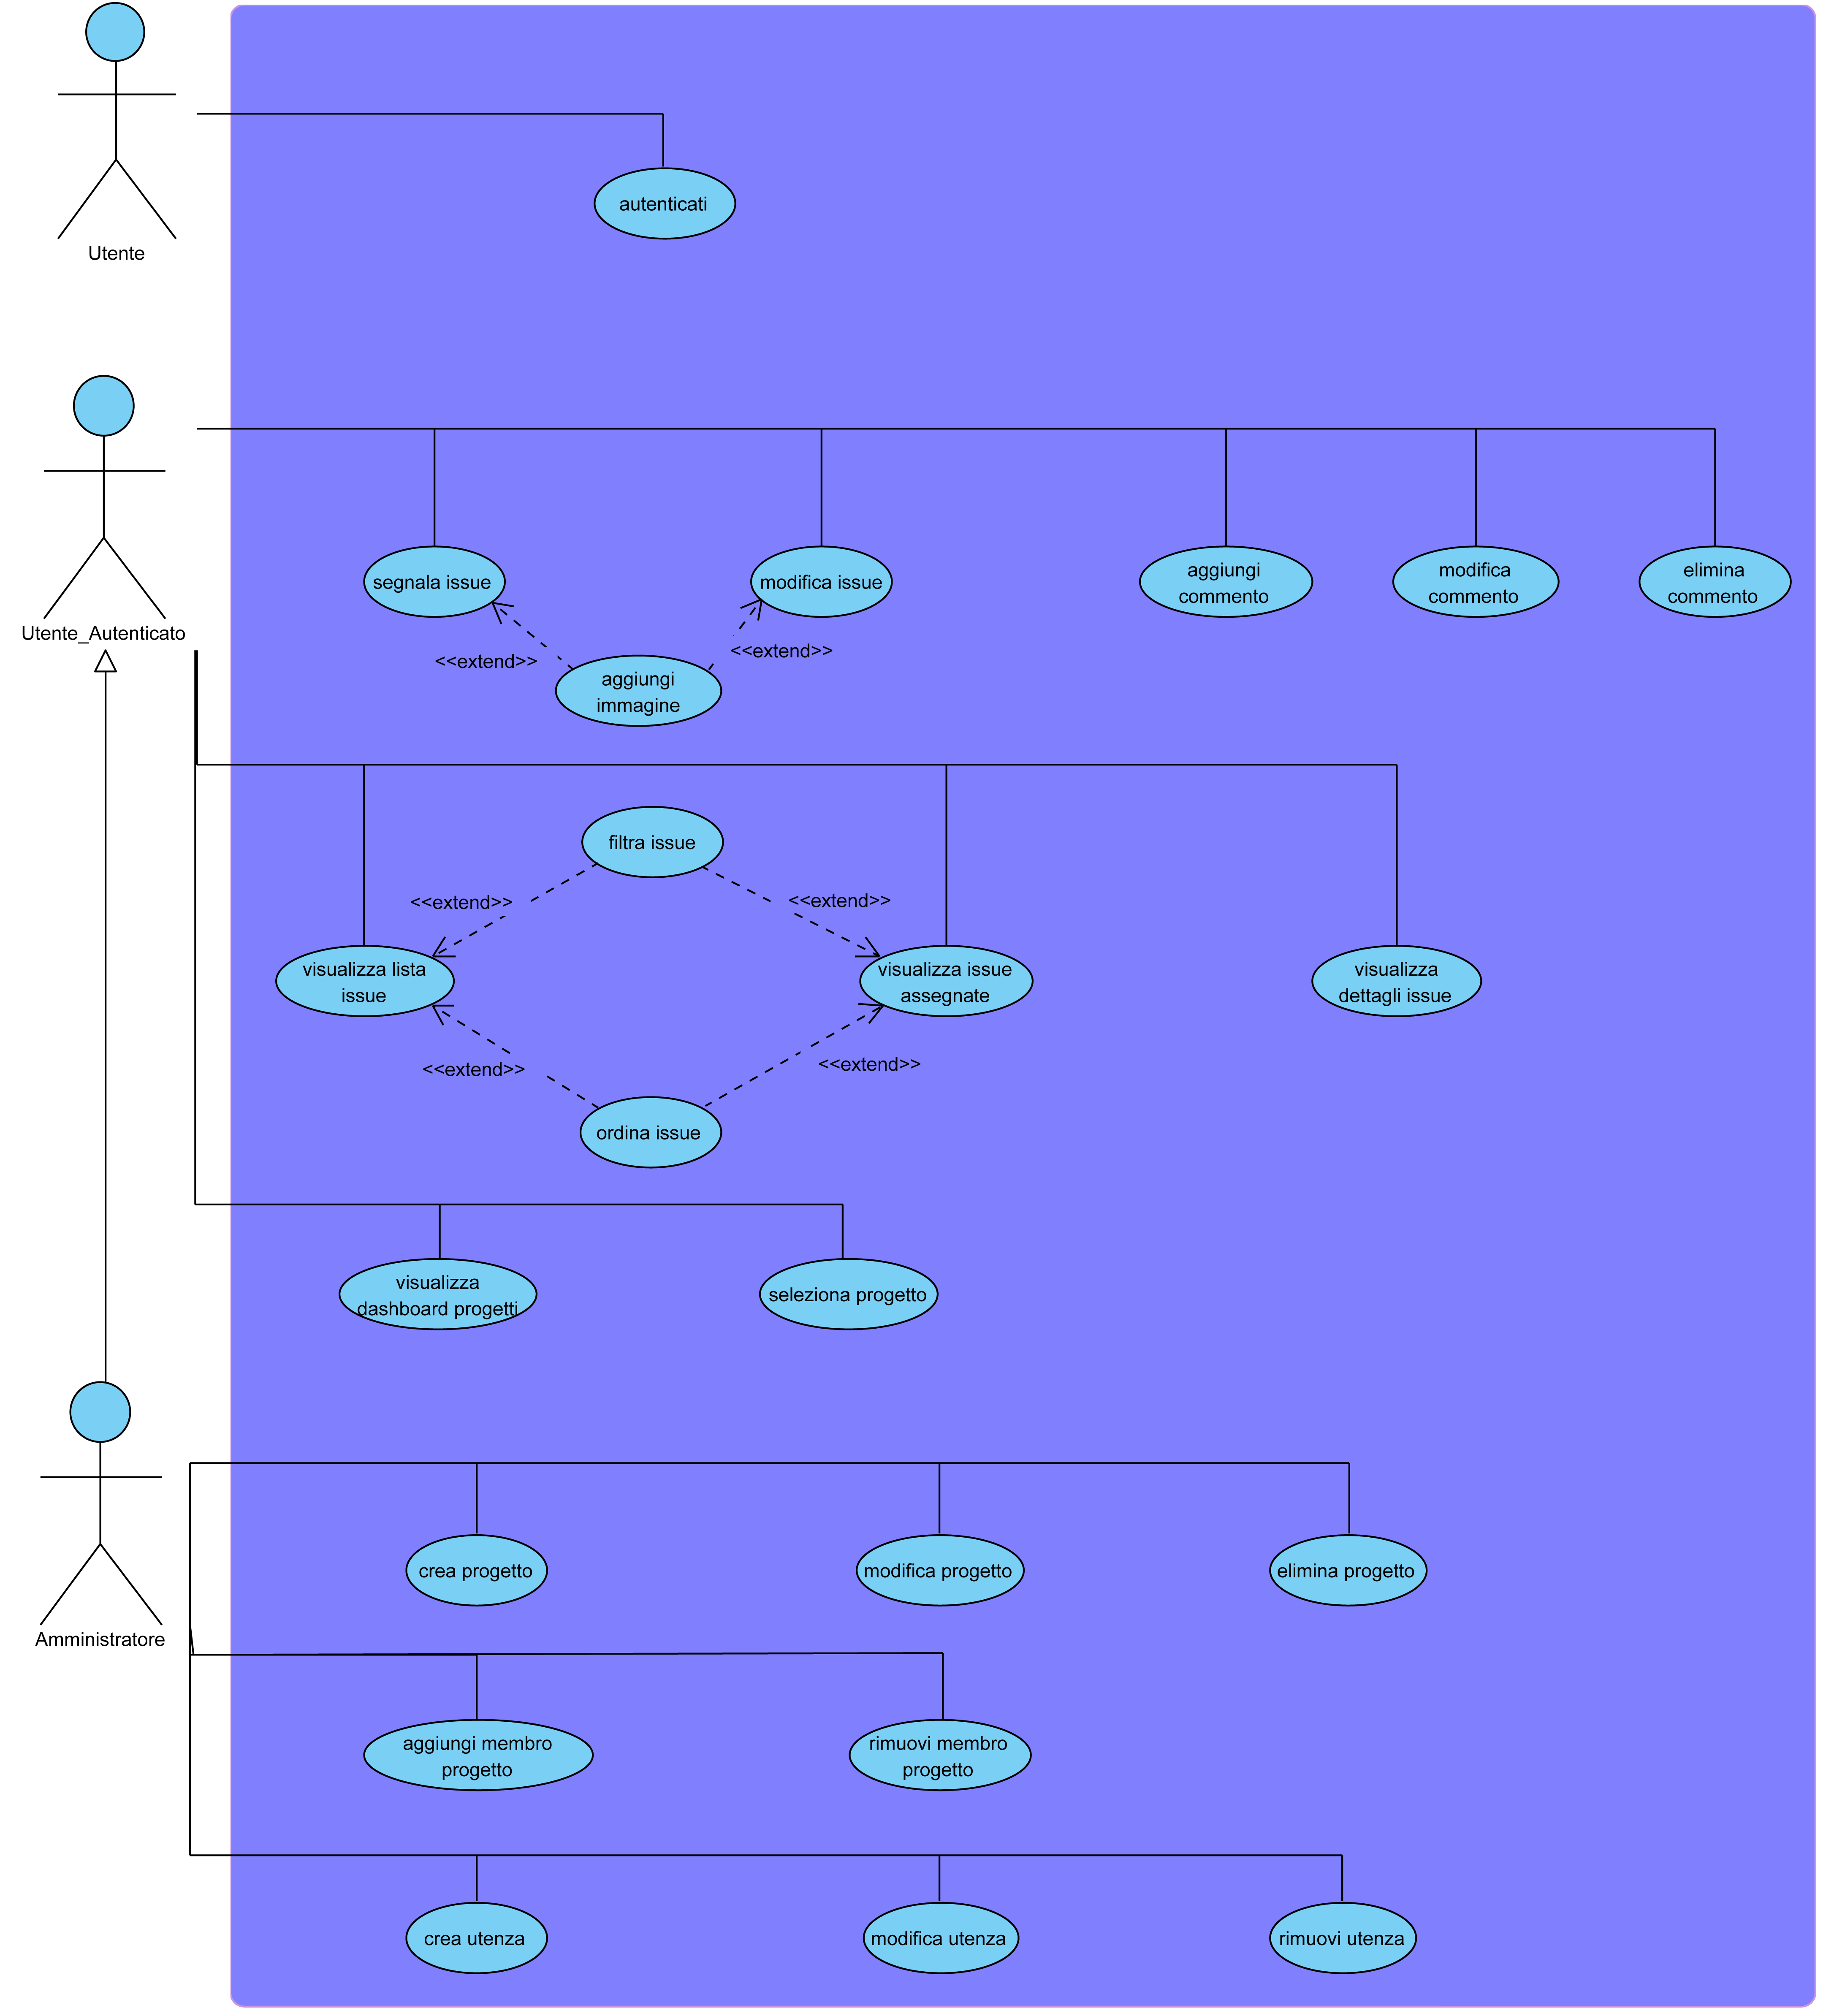
\includegraphics[width=\textwidth]{UCD1.png}
\end{figure}

\textbf{Note sul diagramma}:
\begin{itemize}[leftmargin=1.1em]
\item L'attore \textit{Utente} rappresenta qualunque individuo che accede al sistema prima dell'autenticazione.
\item L'attore \textit{Utente\_Autenticato} eredita implicitamente i permessi di \textit{Utente} e può accedere alle funzionalità di gestione issue.
\item L'attore \textit{Amministratore} eredita tutti i permessi di \textit{Utente\_Autenticato} e dispone di funzionalità privilegiate (gestione utenze, assegnazione, archiviazione, report).
\item Le relazioni \texttt{<<extend>>} indicano funzionalità opzionali che possono essere eseguite in aggiunta al caso d'uso principale.
\end{itemize}

\newpage
% ---------------------------------------------------------------------
\subsubsection{Lista dei casi d'uso}
\label{subsec:lista-use-case}
% ---------------------------------------------------------------------

Sono stati individuati i seguenti casi d'uso per il sistema \productname:

\begin{enumerate}[leftmargin=1.1em]

\item \textbf{UC-01: Autenticazione} \\
\textit{Attore primario}: Utente \\
\textit{Descrizione}: l'utente inserisce email e password per accedere al sistema.

\item \textbf{UC-02: Visualizza Dashboard Progetti} \\
\textit{Attore primario}: Utente Autenticato, Amministratore \\
\textit{Descrizione}: l'utente visualizza la lista dei progetti a cui ha accesso assegnato dall'amministratore, con statistiche e attività recenti per ciascun progetto.

\item \textbf{UC-03: Seleziona Progetto} \\
\textit{Attore primario}: Utente Autenticato, Amministratore \\
\textit{Descrizione}: l'utente seleziona uno dei progetti a cui ha accesso per visualizzarne le issue.

\item \textbf{UC-04: Crea Progetto} \\
\textit{Attore primario}: Amministratore \\
\textit{Descrizione}: l'amministratore crea un nuovo progetto specificando nome, descrizione e membri iniziali del team.

\item \textbf{UC-05: Modifica Progetto} \\
\textit{Attore primario}: Amministratore \\
\textit{Descrizione}: l'amministratore modifica nome, descrizione o altre proprietà di un progetto esistente.

\item \textbf{UC-06: Elimina Progetto} \\
\textit{Attore primario}: Amministratore \\
\textit{Descrizione}: l'amministratore elimina un progetto e tutte le sue issue associate.

\item \textbf{UC-07: Aggiungi Membri Progetto} \\
\textit{Attore primario}: Amministratore \\
\textit{Descrizione}: l'amministratore aggiunge utenti dal team di un progetto, determinando chi può accedere a quel progetto.

\item \textbf{UC-08: Rimuovi Membri Progetto} \\
\textit{Attore primario}: Amministratore \\
\textit{Descrizione}: l'amministratore rimuove utenti dal team di un progetto, determinando chi non può più accedere a quel progetto.

\item \textbf{UC-09: Segnala Issue} \\
\textit{Attore primario}: Utente Autenticato, Amministratore \\
\textit{Descrizione}: l'utente crea una nuova issue all'interno del progetto correntemente selezionato.

\item \textbf{UC-10: Visualizza Lista Issue} \\
\textit{Attore primario}: Utente Autenticato, Amministratore \\
\textit{Descrizione}: l'utente visualizza tutte le issue del progetto corrente.

\item \textbf{UC-11: Visualizza Dettagli Issue} \\
\textit{Attore primario}: Utente Autenticato, Amministratore \\
\textit{Descrizione}: l'utente visualizza il dettaglio completo di una issue del progetto corrente.

\item \textbf{UC-12: Modifica Issue} \\
\textit{Attore primario}: Utente Autenticato, Amministratore \\
\textit{Descrizione}: l'utente modifica attributi di una issue esistente nel progetto.

\item \textbf{UC-13: Aggiungi Etichette} \\
\textit{Attore primario}: Utente Autenticato, Amministratore \\
\textit{Descrizione}: l'utente associa etichette a una issue per categorizzazione.

\item \textbf{UC-14: Aggiungi Immagine} \\
\textit{Attore primario}: Utente Autenticato, Amministratore \\
\textit{Descrizione}: l'utente allega immagini a una issue.

\item \textbf{UC-15: Filtra Issue} \\
\textit{Attore primario}: Utente Autenticato, Amministratore \\
\textit{Descrizione}: l'utente applica filtri per visualizzare sottoinsiemi di issue del progetto.

\item \textbf{UC-16: Ordina Issue} \\
\textit{Attore primario}: Utente Autenticato, Amministratore \\
\textit{Descrizione}: l'utente ordina la lista issue secondo criteri specificati.

\item \textbf{UC-17: Visualizza Issue Assegnate} \\
\textit{Attore primario}: Utente Autenticato, Amministratore \\
\textit{Descrizione}: l'utente visualizza solo le issue del progetto corrente che gli sono state assegnate dall'amministratore.

\item \textbf{UC-18: Aggiungi Commento} \\
\textit{Attore primario}: Utente Autenticato, Amministratore \\
\textit{Descrizione}: l'utente aggiunge commenti testuali a una issue.

\item \textbf{UC-19: Elimina Commento} \\
\textit{Attore primario}: Utente Autenticato, Amministratore \\
\textit{Descrizione}: l'utente elimina i propri commenti.

\item \textbf{UC-20: Visualizza Notifiche} \\
\textit{Attore primario}: Utente Autenticato, Amministratore \\
\textit{Descrizione}: l'utente visualizza notifiche ricevute (assegnazioni, menzioni, aggiornamenti).

\item \textbf{UC-21: Prendi Visione Notifica} \\
\textit{Attore primario}: Utente Autenticato, Amministratore \\
\textit{Descrizione}: l'utente marca le notifiche come lette.

\item \textbf{UC-22: Creazione Utenze} \\
\textit{Attore primario}: Amministratore \\
\textit{Descrizione}: l'amministratore crea nuovi account utente.

\item \textbf{UC-23: Modifica Utenze} \\
\textit{Attore primario}: Amministratore \\
\textit{Descrizione}: l'amministratore modifica dati di account esistenti.

\item \textbf{UC-24: Rimozione Utenze} \\
\textit{Attore primario}: Amministratore \\
\textit{Descrizione}: l'amministratore elimina account utente.

\item \textbf{UC-25: Assegna Issue} \\
\textit{Attore primario}: Amministratore \\
\textit{Descrizione}: l'amministratore assegna una issue a un membro del team del progetto.

\item \textbf{UC-26: Archivia Issue} \\
\textit{Attore primario}: Amministratore \\
\textit{Descrizione}: l'amministratore archivia una issue mantenendone la tracciabilità.

\item \textbf{UC-27: Visualizza Report Mensile} \\
\textit{Attore primario}: Amministratore \\
\textit{Descrizione}: l'amministratore visualizza report mensile con metriche del progetto selezionato.

\end{enumerate}

\newpage